\documentclass{article}
\usepackage{amsfonts}          % Para las negrita de pizarra
\usepackage{indentfirst}       % Para que quede mas lindo el formateo
\usepackage{graphicx}          % Para graficos
\usepackage{minted}            % Para poner codigo y que quede con sintaxis fachera
\usepackage{hyperref}          % Para meter hipervinculos
\usepackage[dvipsnames]{xcolor}% Para usar colores
\usepackage{hhline}            % Mas configuracion para las líneas en tablas
\usepackage{amsmath}           % Agregado para tags de ecuaciones
\usepackage{xcolor}            % Coloreado de ecuaciones
\usepackage{quoting, xparse}   % Usado para citar
% \usepackage{svg}               % Para usar imagenes svg que se ven lindas independientemente del zoom. WARNING REQUIERE DE INKSCAPE. Tal vez no vale la pena
\usepackage{amsmath}

\graphicspath{ {./images/} }

\newcommand{\docuPy}{%
  {\href{https://wiki.python.org/moin/TimeComplexity}{documentación oficial}}
  }%

  % Comandos para facilitar el citado
  % Fuente: https://tex.stackexchange.com/a/391739/273865
\NewDocumentCommand{\bywhom}{m}{% the Bourbaki trick
  {\nobreak\hfill\penalty50\hskip1em\null\nobreak
   \hfill\mbox{\normalfont(#1)}%
   \parfillskip=0pt \finalhyphendemerits=0 \par}%
}

\begin{document}

\begin{titlepage}
  \vspace*{1cm}

  \begin{center}
    {\Huge{Trabajo Práctico 3: Problemas NP-Completos para la defensa de la Tribu del Agua}}
  \end{center}

  \vspace{0.4cm}

  \begin{center}
    {\LARGE{Facultad de Ingeniería de la Universidad de Buenos Aires}}\\
    \vspace{0.3cm}
    {\Large{Teoría de Algoritmos}}\\
    \vspace{0.3cm}
    {\large{Cátedra Buchwald-Genender}}\\
  \end{center}

  \vspace{0.8cm}
  \begin{center}
    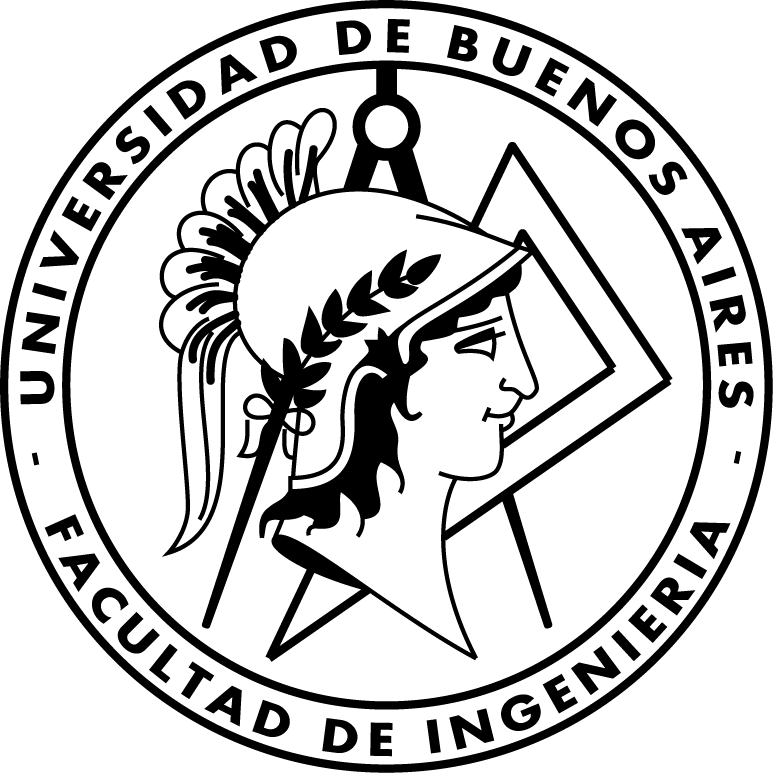
\includegraphics[scale=0.8]{Logo-fiuba}
  \end{center}

  \vspace{1.4cm}
  \begin{center}

    {\begin{minipage}[t]{.32\textwidth}
        \begin{center}
          Gómez Belis, Sofía\\
          {\small{Padrón: 109358}}\\
          {\small{email: sgomezb@fi.uba.ar}}
        \end{center}
          \end{minipage}
          \begin{minipage}[t]{.32\textwidth}
        \begin{center}
          Llanos Pontaut, Valentina\\
          {\small{Padrón: 104413}}\\
          {\small{email: vllanos@fi.uba.ar}}\\
        \end{center}
      \end{minipage}
      \begin{minipage}[t]{.32\textwidth}
        \begin{center}
          Orsi, Tomas Fabrizio\\
          {\small{Padrón: 109735}}\\
          {\small{email: torsi@fi.uba.ar}}
        \end{center}
      \end{minipage}}

  \end{center}
\end{titlepage}

\renewcommand*\contentsname{Indice}
\tableofcontents
\pagebreak

\section{Introducción}
\subsection{Descripción y objetivo}
\label{sec:descripcion}

Continuando con el ataque de la Nación del Fuego sobre el resto de las naciones, esta vez es la Tribu del Agua la que requiere de nuestra ayuda para defenderse. 

Cada maestro agua tiene una fuerza o habilidad positiva $x_i$, y contamos con el conjunto de todos los valores $(x_i, x_2, \dots, x_n)$. Basándonos en estos, el maestro Pakku desea separar los maestros en \texttt{k} grupos $(S_1, S_2, \dots, S_k)$ parejos tal que cuando un grupo se canse, entrará el siguiente en el combate, obteniendo un ataque constante que les permita salir victoriosos, aprovechando también la ventaja del agua por sobre el fuego.

Para que los grupos estén lo más parejos posibles, nos han encomendado minimizar la adición de los cuadrados de las sumas de las fuerzas de los grupos:

$$
\min \sum_{i=1}^{k} \left( \sum_{x_j \in S_i} x_j \right)^2
$$

En este trabajo desarrollaremos algoritmos de backtracking, programación lineal y posibles aproximaciones buscando resolver el problema planteado con el objetivo de ayudar a los maestros de la Tribu del Agua a derrotar a la Nación del Fuego.

\section{Demostración de problema NP-Completo}
\label{sec:np-completo}

Los problemas NP-Completos son los problemas más difíciles de NP. Cualquier problema en NP puede ser reducido a uno NP-Completo.

Para demostrar que el problema de la Tribu del Agua es NP-Completo, primero debemos demostrar que se encuentra en NP. Posteriormente, si logramos hacer una reducción polinomial de un problema NP-Completo a éste, entonces esto implica que también se trata de un problema NP-Completo. Ésto se debe a que la reducción $Y \leq_p X$ implica que la dificultad de resolver \texttt{Y} se reduce polinomialmente a la dificultad de resolver \texttt{X}, o que \texttt{X} es al menos tan difícil de resolver como \texttt{Y}. Si \texttt{Y} es un problema NP-Completo, entonces \texttt{X} es al menos tan difícil de resolver como un problema NP-Completo.

Para realizar la demostración y la reducción, necesitamos basarnos en el problema de decisión:

Dados una secuencia de \texttt{n} fuerzas de maestros agua $(x_i, x_2, \dots, x_n)$, y dos números \texttt{k} y \texttt{B}, ¿existe una partición en \texttt{k} subgrupos $(S_1, S_2, \dots, S_k)$ tal que:

$$
\sum_{i=1}^{k} \left( \sum_{x_j \in S_i} x_j \right)^2 \leq B
$$

y cada elemento $x_i$ esté asignado a solamente un grupo?
\subsection{Problema en NP}

Un problema se encuentra en NP si existe un certificador eficiente para el mismo. Es decir, si puede ser verificado o validado en tiempo polinomial. 

Tenemos los siguientes datos:
\begin{itemize}
    \item Habilidades de los maestros $\rightarrow$ se presentan en forma de tupla (nombre maestro, fuerza)
    \item Cantidad de subconjuntos $\rightarrow$ \texttt{k}
    \item Cota del coeficiente $\rightarrow$ \texttt{B}
    \item Resultado a validar $\rightarrow$ subconjuntos $S_i$ que contienen los nombres de los maestros del grupo correspondiente
\end{itemize}

También tenemos las siguientes restricciones:
\begin{itemize}
    \item Cada maestro debe estar asignado a un solo grupo
    \item El resultado debe contener \texttt{k} grupos
    \item La sumatoria resultante debe ser a lo sumo \texttt{B} 
\end{itemize}

Dados estos datos y restricciones, proponemos el siguiente certificador.
\inputminted[linenos, firstline=1, lastline=31]{python}{codigo/certificador_eficiente.py}

Para que el verificador presentado pueda ser considerado un certificador eficiente, debe ejecutarse en tiempo polinomial. Por lo tanto, procedemos a explicar y justificar la complejidad del código.

Realizamos operaciones aritméticas, asignaciones y verificaciones. Todas estas son operaciones $O(1)$ puesto que consumen tiempo constante según la \docuPy. Recorremos dos veces la lista de maestros y habilidades con diferentes propósitos. Como contiene \texttt{n} tuplas, cada ciclo \texttt{for} tiene un costo $O(n)$. Con el objetivo de obtener la adición de los cuadrados de las sumas de las fuerzas de los grupos y compararla con \texttt{B}, tenemos dos ciclos anidados. El segundo recorre los maestros de un grupo que, en el peor caso, son \texttt{n}. Esto se realiza \texttt{k} veces, por lo que en total es $O(k \times n)$.

Entonces,

$$
T(n) = O(1) + 2 \cdot O(n) + O(k \times n) = O(k \times n)  
$$

En el peor caso, $k = n$ y

$$
T(n) = O(n \times n) = O(n^2)
$$

Ambas cotas, $O(k \times n)$ y $O(n^2)$ conllevan tiempo polinomial. Por lo tanto, podemos afirmar que existe un certificador eficiente para el problema de la Tribu del Agua y entonces este problema está en NP.

\subsection{Problema 2-Partition}

Para demostrar que el problema de la tribu del agua es NP-Completo haremos uso del problema 2-Partition. Este se define de la siguiente manera: se tiene un conjunto de n elementos, cada uno con un valor, y se desea separarlos en 2 subconjuntos tal que la suma de los valores de cada uno sea igual para ambos. Procederemos a justificar que se trata de un problema NP-Completo.

\subsubsection{Problema en NP}
Enunciamos el problema de decisión asociado: dado un conjunto \( \{a_1, a_2, \ldots, a_n\} \), ¿existen dos subconjuntos \( S_1 \) y \( S_2 \) tales que \( \sum_{x \in S_1} x = \sum_{x \in S_2} x \)?

A continuación mostramos la implementación de un validador:
\inputminted[linenos]{python}{codigo/certificador_2_partition.py}

Hay tres ciclos \texttt{for}. Uno de ellos recorre todos los valores del conjunto. Considerando que hay \texttt{n}, es una operación $O(n)$. Los conjuntos $S_1$ y $S_2$ deberían contener en total $n$ elementos, pudiendo uno de ellos tener hasta  $n-1$. En total, ambos conllevan $O(n)$. Por lo tanto, la complejidad temporal del validador es $O(n)$, constituyendo un certificador eficiente. Como el problema 2-Partition puede ser verificado en tiempo polinomial, podemos afirmar que se encuentra en NP.

\subsubsection{Reducción}
\label{sec:np-completo-2p}

Como hemos visto en clase, el problema de subset sum es NP-Completo. Utilizaremos esta conclusión para demostrar que 2-Partition también lo es.

Dado un conjunto de números \( S = \{a_1, a_2, \ldots, a_n\} \) y un número \( B \), queremos saber si hay un subconjunto de \( S \) cuya suma sea igual a \( B \).

Para realizar la reducción $SS \leq_p 2P$, debemos definir cuál es la entrada (conjunto) de la caja negra que resuelve 2-Partition. Sea $s = sum(S)$ la suma de los valores del conjunto $S$, definimos \( S' = S \cup \{s - 2\cdot B\} \). Aplicamos el algoritmo en $S'$.

Si \( T \subseteq S \) es un subconjunto con suma \( B \):

\begin{itemize}
    \item Sea \( O = S \setminus T \), con suma \( o = s - B \), los elementos que ``sobran''.
    \item Sea \( T' = T \cup \{s - 2 \cdot B\} \), cuya suma es \( B + (s - 2 \cdot B) = s - B \). Es el subconjunto buscado, unido con el valor agregado a $S$.
    \item $ O \cup T' = S'$
\end{itemize}

Entonces, la suma de \( T' \) y \( O \) es la misma, \( s - B \), lo que significa que podemos dividir \( S' \) en dos subconjuntos con la misma suma.

Luego, existe un subset sum de valor $B$ en $S$ si y solo si existe un 2-Partition en $S'$:

    $\rightarrow$ Si existe un conjunto de números en $S$ que suman $B$, entonces los números restantes en $S$ suman \(s - B\). Por lo tanto, existe una partición de \texttt{S'} en dos tal que cada partición suma \(s - B\): \( O = S \setminus T \) y \( T' = T \cup \{s - 2 \cdot B\} \). 

    $\leftarrow$ Digamos que existe una partición de \texttt{S'} en dos conjuntos tal que la suma de cada conjunto es \(s - B\). Uno de estos conjuntos contiene el número \(s - 2 \cdot B\). Eliminando este número, obtenemos un conjunto de números cuya suma es $B$, y todos estos números están en $S$.

Como esta reducción conlleva una transformación polinomial, podemos afirmar que 2-Partition es un problema NP-Completo.

Ejemplo 1: La entrada de Subset Sum es \( S = \{3, 1, 4, 2, 2\} \) y \( B = 6 \). Como la suma de los valores de $S$ es 12, agregamos el elemento $12 - 2 \cdot 6 = 0$ \( S' = \{3, 1, 4, 2, 2, 0\} \). Este conjunto puede ser particionado en \( \{3, 1, 2\} \) y \( \{4, 2, 0\} \), ambas con suma 6, donde \( T = \{3, 1, 2\} \) es un subconjunto de \( S \) que suma \( 6 \). Por lo tanto, la caja negra que resuelve el problema de partición, nos devolverá que es posible encontrar un subset sum que sume $B$.

Ejemplo 2: La entrada de Subset Sum es \( S = \{5, 3, 2, 7\} \), que suma 17, y \( B = 10 \). Agregamos el valor $17 - 2 \cdot 10 = -3$. Entonces, \( S' = \{5, 3, 2, 7, -3\} \) y se puede dividir en  \( \{7\} \) y \( \{2, 5, 3, -3\} \), donde \( T = \{2, 5, 3\} \) es el subconjunto que suma \( 10 \). Nuevamente existe solución. En cambio, si $B = 6$, tendríamos \( S' = \{5, 3, 2, 7, 5\} \) no puede dividirse en dos subconjuntos que sumen $22 \over 2 = 11$, por lo que no existirá un subset sum con $B = 6$ en $S$.

\subsection{Reducción del Problema del Balanceo de Carga}
\subsubsection{Introducción}
Habiendo establecido que el problema pertenece a NP, ahora vamos a realizar una reducción de un problema NP-Completo a este problema.
Para esta reducción, decidimos reducir el problema del Balanceo de Carga (que llamaremos B.C.) al problema de la tribu del agua (que llamaremos T.A.). Esto es decir, nuestra reducción polinomial va a ser de la forma:
$$
BC \leq_p TA
$$

BC plantea lo siguiente: 
\textit{Dadas m Máquinas y un conjunto n de trabajos, donde cada trabajo j toma un tiempo Tj, se desea asignar el trabajo en las Máquinas de forma balanceada. Dada una asignación A(i) para la Máquina i, su tiempo de trabajo es: $T_{i} =\displaystyle{\sum_{j \in A(i)} t_j}$. Y queremos encontrar la asignación que minimice el máx valor de Ti, que también representa el tiempo que se tardará en finalizar todos los trabajos.}

Si escribimos en forma de ecuación lo que plantea BC, obtenemos la siguiente expresión:
$$
\min( \max (\displaystyle{\sum_{j \in A(i)} t_j}))
$$

La versión de decisión de este problema dice: Dado un numero $m$ de maquinas, una serie $n$ de trabajos, y un numero $C$, determinar si existe un asignación de trabajos en las $m$ maquinas, tal que el máximo $T_i$ sea menor o igual a $C$.

Cabe destacar que en clase nosotros estudiamos al problema de BC como un problema NP-Hard; resta aun demostrar que es un problema NP-Completo. Vamos a resolver esto en la próxima sección.

\subsubsection{Demostración de problema NP-Completo}
\label{sec:np-completo-bc}
Para demostrar que BC es un problema NP-Completo, vamos a usar el problema 2P (el cual demostramos que es NP completo en \nameref{sec:np-completo-2p}). Es decir que vamos a realizar la reducción
$$
2P \leq_p TA
$$

Nosotros partimos de una serie de números $S = \{a_1, a_2, \ldots, a_n \}$. Por cada numero $a_i$ definimos un trabajo $n$ con duración $a_i$.  
Luego, por cada uno de los dos subconjunto $S_i$, definimos una maquina $m_i$.
Finalmente, decimos que nuestros valor $C$ va a ser la mitad de la suma de todos los $a_i$.

Cuando le pasemos este nuevo problema al validador de BC, este nos va a decir si es posible partir el conjunto en dos subconjuntos. Esto se debe a que solo va a ser posible partir el conjunto en dos si como mucho, cada subconjunto tiene exactamente la mitad de la suma. 

Con esto mostramos que el problema BC es un problema NP-Completo.





\subsubsection{Desarrollo}
El problema de decisión de BC, busca minimizar el máximo valor de las maquinas; mientras que TA busca lograr que todos los subgrupos tengan una duración pareja. La pregunta entonces es: ¿Hay relación entre estas dos búsquedas?. ¡La respuesta es que si! Buscar minimizar el máximo valor de las maquinas, está implícitamente buscando lograr que todas las máquinas tengan una duración pareja.
Para reducir el tiempo de uso de una maquina, se le tiene que dar alguno de sus trabajos a otra máquina. Cuanto mas trabajos se pueda pasar a otra maquina (sin que esta se convierta en la nueva maquina de mayor duración), mas voy a lograr minimizar el valor máximo de las maquinas.
Esto implica que en el momento que se tenga todas las máquinas con igual $T_i$, es el momento en donde va a estar el mínimo valor máximo de $T_i$. Esto se ve en que si una maquina le da un trabajo a otra, una maquina va a estar por debajo de todas las anteriores, pero la otra va a tener un valor por encima de todas estas. Esto implica un mayor nivel máximo de $T_i$.

Basándonos, podemos realizar la siguiente reducción:
Por cada trabajo $n_i$, definimos un maestro agua $x_i$. Por cada máquina $m_i$ definimos un subgrupo $S_i$ ($m$ sería nuestro $k$).
Luego tenemos $C$, el cual representa una cota máxima para el máximo valor de $T_i$. Para transformarlo a $B$ en tiempo polinomial, tenemos que elevar $C$ al cuadrado y sumarle a este nuevo valor todo los otros valores de $T_i$ al cuadrado. Esto nos va a dar una cota equivalente al problema de decisión de TA.
Entonces, después de realizar estas transformaciones, le tenemos que pasar esta instancia de problema al validador de problemas de TA, el cual nos va a decir si la solución es válida o no.

\section{Complejidad algorítmica}
\subsection{Complejidad lectura de archivos}
\subsection{Complejidad algoritmo de Backtracking}
\subsection{Complejidad algoritmo de programación lineal}
\subsection{Complejidad algoritmo de aproximación}

\subsection{Efecto de las variables sobre el algoritmo}

\section{Ejemplos de ejecución}
\label{sec:ejemplos}
\section{Mediciones de tiempo}
\label{sec:medTiempo}
\subsection{Algoritmo de backtracking}
\subsection{Algoritmo de programación lineal}
\subsection{Algoritmo de aproximación}


\section{Conclusión}


\end{document}
